\documentclass[a4paper,11pt]{article}

% Preamble
\input{../../shared/preamble.pty}

% Hyperref settings
\hypersetup{
    colorlinks=true,
    linkcolor=blue,
    filecolor=magenta,
    urlcolor=cyan,
    pdftitle={Polycentric Voting (PV)},
    pdfauthor={Samuel J. Gosling},
    pdfsubject={Governance, Economics},
    pdfkeywords={weighted voting, polycentrism, polycracy, plutocracy, governance, voting power}
}

\begin{document}
\begin{center}
{\huge \textbf{Polycentric Voting (PV)}} \\[2em]
{\large \fontseries{sb}\selectfont Samuel J. Gosling} \\[.2em]
{\large {samuel@focal.org}} \\[1em]
{\large \today}
\end{center}

\section*{Abstract}

\vspace{1em}
\begin{mdframed}[
  linewidth=190000sp,
  linecolor=black,
  topline=false,
  bottomline=false,
  rightline=false,
  innerleftmargin=14pt,
  innerrightmargin=1pt,
  innertopmargin=0pt,
  innerbottommargin=-0.5pt
]
{\small\fontseries{sb}\selectfont A progressive voting model that introduces time and commitment as independent axes of authority beyond capital in contrast to traditional shareholder governance where all votes are weighted identically regardless of tenure, which systematically favours short-term actors. A path-dependent time weight captures the trajectory of commitment rather than a snapshot of individual holdings and normalising influence across graduated phases through discrete power tranches. This produces emergent demographic stratification that satisfies both Polanyi's structural definition of polycentrism and Ostrom's empirical conditions for effective collective governance, a formal resolution to the misalignment between capital markets and long-term institutional interests.}
\end{mdframed}

\section{Background}
\begin{multicols}{2}
\raggedright
Authority in organisational governance is typically denominated by shares or tokens. One-share one-vote systems enable decisive decision-making but concentrate power among wealthy stakeholders, creating vulnerability to vote-buying and marginalising smaller participants - eroding representation and increasing systemic exposure to short-sighted governance. \newline \\ \textbf{Penrose (1946)} first proposed the square-root method as a means of saturating concentrations of power while preserving broad representation, laying the mathematical foundation for modern weighted voting theory. Writing in relative obscurity, his contribution went largely unrecognised for decades - the square-root function he identified as the natural basis for fair weighted voting has not found relevance until the present work. 

\textbf{Polanyi (1951)} philosophised the thesis of polycentrism - cooperative bodies with multiple nodes of authority where no single actor maintains complete control. Plutocracy presents the impression of a polycentric system through dispersed ownership yet mechanically collapses into hierarchy, as capital accumulation faces no structural resistance and authority reduces to a single axis. \newline \\  \textbf{Ostrom (1990)} demonstrated that the design of governance institutions fundamentally determines the success of collective action - carefully crafted rules enable effective autonomous governance without requiring continuous external intervention. The design challenge remains: how to equitably balance influence, commitment, and protection from manipulation without compromising a governing system's capacity to adapt and act.
\end{multicols}

\section{Theory}

\subsection{Effective Time Weight}

When quantifying time the optimal solution relies in progressively scaling the multiplier proportional to base average voting power, this is done to promote behaviour of either absolute (singleton) or progressive power accumulation (sequential), see section 3.5. Where $t_d$ is the delta time factor following unix time, $a_i$ equates to an increment amount of shares held or deposited.

\begin{equation}
t_{\text{effective}} = \frac{\sum a_i \cdot t_d}{\sum a_i}    
\end{equation}

In cases of rebalancing the time weight, we use the derivative notation to represent delta change: 

\begin{equation}
{t'}_{\text{effective}} = \frac{\sum a_i \cdot t_d - {a_d \cdot t_{\text{effective}} }}{\sum a_i - a_d}    
\end{equation}

\subsubsection{Addition}

This introduces the time multiplier being diluted with the introduction of additional shares, the proportion of which is equal to the active share amount. For example, Bob has a balance of 1000 shares with an effective time weight of 100 days. Bob decides to deposit an additional 500 shares, which dilutes his effective time weight to 66.7 days, a reduction of 33.3\%.  

\vspace{5pt}

\subsubsection{Subtraction}

However, in the case of withdrawing or removing shares, the effective time weight is preserved in order to not disenfranchise committed stakeholders given that the share balance is a non-zero value, where $a_w$ represents the withdrawal amount. 

\subsubsection{Path-dependency}
The variance of $t_{\text{effective}}$ is produced by the scalar product of deposit amounts and time deltas across the shareholders profile is defined as:

$$\rho = \text{Var}(\{t_{\text{effective}_i}\}_{i = 1}^{n})$$

Where higher $\rho$ reflects greater divergence in commitment, therefore tenure ($\tau$) can be defined as:

$$\tau \propto \frac{1}{\rho}$$

A consistent trajectory produces low $\rho$ and high $\tau$, whereas irregular commitment history results anomalously high $\rho$ and thus low $\tau$, acting as the product of a shareholder's \textbf{commitment profile}.

\subsection{Power Levels}

Using predefined tranches ($P$), defined as $0 \leq P \leq 1$ and dependent on $t_{\text{effective}}$, translates natural bands or levels across the voting power curve, creating distinct tiers or stages to the governance lifecycle. The default preference defines five discrete power levels with base tranche values: $P_1 = 0.2$ (new), $P_2 = 0.4$ (early), $P_3 = 0.6$ (median), $P_4 = 0.8$ (mature), and $P_5 = 1.0$ (veteran).

\vspace{5pt}

\begin{equation}
P_{\text{culm}}(t_{\text{effective}}) = \begin{cases}
0.2 & \text{if } t_{\text{effective}} < 30 \\
0.6 & \text{if } 30 \leq t_{\text{effective}} < 90 \\
1.2 & \text{if } 90 \leq t_{\text{effective}} < 180 \\
2.0 & \text{if } 180 \leq t_{\text{effective}} < 365 \\
3.0 & \text{if } t_{\text{effective}} \geq 365
\end{cases}
\end{equation}

\vspace{15pt}

Which are cumulatively aggregated as $P_{\text{culm}}$ for efficient lookup in O(1) time complexity,  result in voting power becoming normalised across these phases of governance, requiring cross-consensus for effective decision-making and ultimately creating a more nuanced governance process. 

\subsection{Time Weight}

Given the effective time weight $t_{\text{effective}}$, the time weight is computed using precomputed cumulative tranche coefficients for optimal computational efficiency.

\vspace{5pt}

\begin{equation}
    W = P_{\text{culm}}(t_{\text{effective}}) \cdot t_{\text{effective}}
\end{equation}

\vspace{15pt}

Where $P_{\text{culm}}(t_{\text{effective}})$ is determined by tranche lookup, maintaining identical power progression as summation while achieving O(1) complexity.

\subsection{Power Ratio}
The power ratio is the proportion of quadratic to linear in the weighting of voting power, in PV being dependent on time ($t$) but in theory can be applied to any arbitrary metric.

\vspace{5pt}

\begin{equation}
    \alpha = \max(r_{\min}, \min(r_{\max}, r_{\max} + ( t_{\text{effective}} \cdot k)))
\end{equation}

\vspace{15pt}

Where $\alpha = 1$ equates to fully linear weighting and $\alpha = 0$ to entirely quadratic weighting, with variable $k$ being defined as time limiting factor.

\vspace{5pt}

\begin{equation}
    k = \frac{r_{\max}}{\log_2(t_{\max})}
\end{equation}

\vspace{15pt}

Where $t_{\max}$ is defined as the time value for maturity, here defined as 730 days or 24 months, using lograthmic time to provide diminishing returns over-time.

\subsection{Voting Power}

Where $T$ is token amount, $W$ is time weight, and $\alpha$ is the power ratio.

\vspace{5pt}

\begin{equation}
    V_P = W(\alpha \cdot T + \sqrt{T}(1-\alpha))
\end{equation}

\section{Power Analysis}

To replicate a more realistic distribution, shareholder actors from each tier are added gradually over 80 day period to portray the temporal dynamics of voting power when bootstrapping a governing body. Share distribution features tiered holder structure with factor-based scaling (4x, 2x, 1x, 0.4x, 0.1x) ensuring governance representation across wealth demographics for realistic assumptions with team cooperation and market liquidity.

\vspace{10pt}

\begin{table}[h!]
\centering

% --- Full-width distribution table ---
\begin{tabularx}{\textwidth}{>{\bfseries}l >{\bfseries}X >{\centering\arraybackslash}X 
                                     >{\centering\arraybackslash}X 
                                     >{\centering\arraybackslash}X 
                                     >{\centering\arraybackslash}X}
\toprule
\textbf{Category} & \textbf{Tier} & \textbf{Shares per} & \textbf{Count} & \textbf{Total} & \textbf{Percent} \\
\midrule
\multirow{5}{*}{Stakeholders}
 & Major  & 2,000 & 5  & 10,000 & 10.0\% \\
 & Large  & 1,000 & 10 & 10,000 & 10.0\% \\
 & Median & 500   & 20 & 10,000 & 10.0\% \\
 & Minor  & 200   & 40 & 8,000  & 8.0\% \\
 & Small  & 50    & 40 & 2,000  & 2.0\% \\
\cmidrule(lr){2-6}
 & \textit{Subtotal} & – & 115 & 40,000 & 40.0\% \\
\midrule
Operations & – & 40,000 & 1 & 40,000 & 40.0\% \\
Liquidity  & – & 20,000 & 1 & 20,000 & 20.0\% \\
\midrule
\textbf{Total Supply} & – & – & 117 & 100,000 & 100.0\% \\
\bottomrule
\end{tabularx}

\vspace{-.15em}

% --- Full-width onboarding schedule ---
\begin{tabularx}{\textwidth}{l*{6}{>{\centering\arraybackslash}X}}
\toprule
\textbf{Day} & \textbf{Major} & \textbf{Large} & \textbf{Median} & \textbf{Minor} & \textbf{Small} & \textbf{Holders} \\
\midrule
0   & 1 & 2 & 3  & 6  & 2  & 14 \\
20  & 2 & 4 & 7  & 14 & 8  & 35 \\
40  & 3 & 7 & 12 & 25 & 18 & 65 \\
60  & 4 & 9 & 17 & 35 & 30 & 95 \\
80  & 5 & 10 & 20 & 40 & 40 & 115 \\
\bottomrule
\end{tabularx}

\caption{Share distribution and schedule}

\label{tab:full_governance_table}
\end{table}

\newpage

\section{Strategies}

\subsection{Singleton}

A stakeholder contributes a singular denomination stake, which results in the most absolute state of voting power accumulation and weight. For example, Bob locks 10,000 shares. A time-capital commitment, with no subsequent withdrawals until maturity.  

\subsection{Sequential}

A stakeholder strategically obtains or locks shares gradually to dilute their time weight at an optimal threshold to allow voting power to compound effectively. For example, Alice locks 3,333 shares and subsequent deposits at; 1,667 shares at 90 days, 2,500 shares at 180 days and 2,500 at 270 days. This results a much more progressive power accumulation but is an operational strategy.  

\subsection{Splitting}

A stakeholder aims to take advantage of the quadratic weighting by sybil attacking. For example, Claude has 10,000 shares and splits the balance to different stakeholder accounts. Amplifying their voting power temporally due to the quadratic weighting.  

\subsection{Benchmark}

Each strategy assumes a total allocation of 10,000 shares, where $P$ equals 0.2 at $t_p$ to 30 days, then 0.4 for 90 days, 0.6 for 180 days, 0.8 for 365 days and 1 for 720 days.

\begin{figure}[h]
    \centering
    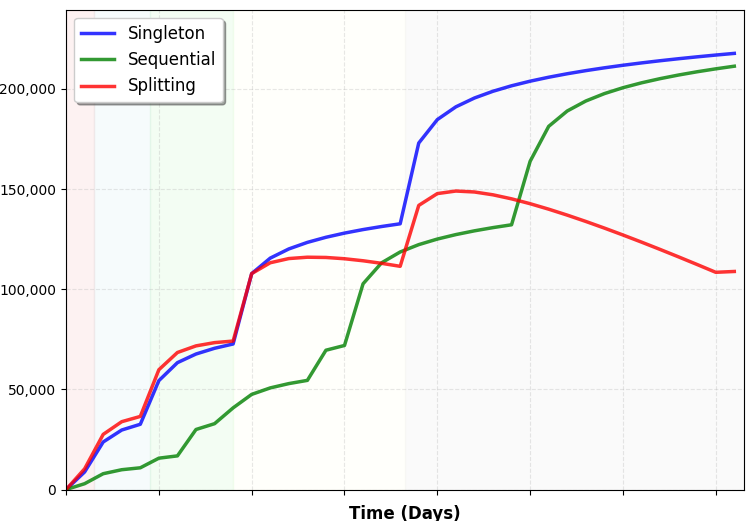
\includegraphics[width=0.8\textwidth]{assets/strategy_vp.png}
    \caption{Strategies voting power series}
    \label{fig:gini}
\end{figure}

\begin{table}[h!]
\centering
\begin{tabularx}{\textwidth}{l*{6}{>{\centering\arraybackslash}X}}
\toprule 
Strategy & 3 Months & 6 Months & 12 Months & 24 Months & Impact \\
\midrule
Singleton & 3,938& 6,563 & 7,884 & 10,000 & +100\% \\
Sequential & 3,360 & 5,888 & 7,792 & 9,400  & +88\% \\
Splitting & 4,860& 6,480& 7,200 & 5,000 & -50\%  \\
\bottomrule
\end{tabularx}
\caption{Strategy voting power}
\label{tab:strategy}
\end{table}

\begin{table}[h!]
\centering
\begin{tabularx}{\textwidth}{l*{5}{>{\centering\arraybackslash}X}}
\toprule 
Strategy & 3 Months & 6 Months & 12 Months & 24 Months & Average \\
\midrule
Singleton & 1,313 $V_{p}$/s & 1,094 $V_{p}$/s & 657 $V_{p}$/s& 417 $V_{p}$/s& 870 $V_{p}$/s \\
Sequential & 1,120 $V_{p}$/s & 981 $V_{p}$/s & 649 $V_{p}$/s & 392 $V_{p}$/s & 786 $V_{p}$/s \\
Splitting & 1,620 $V_{p}$/s & 1,080 $V_{p}$/s & 600 $V_{p}$/s & 208 $V_{p}$/s & 877 $V_{p}$/s \\
\bottomrule
\end{tabularx}
\caption{Strategy power rates}
\label{tab:strategy_rates}
\end{table}

While token-splitting is advantageous in the short-term, it ultimately fails to increase voting power over time but actually expenses a stakeholder's governance influence by approximately 50\% due to the time weighting loss. Following the Nash  equilibrium theorem, we can identify the Singleton strategy as the dominant strategy, the Sequential strategy as the equilibrium strategy and the Splitting strategy as the suboptimal strategy.

\section{Results}

\begin{figure}[h]
    \centering
    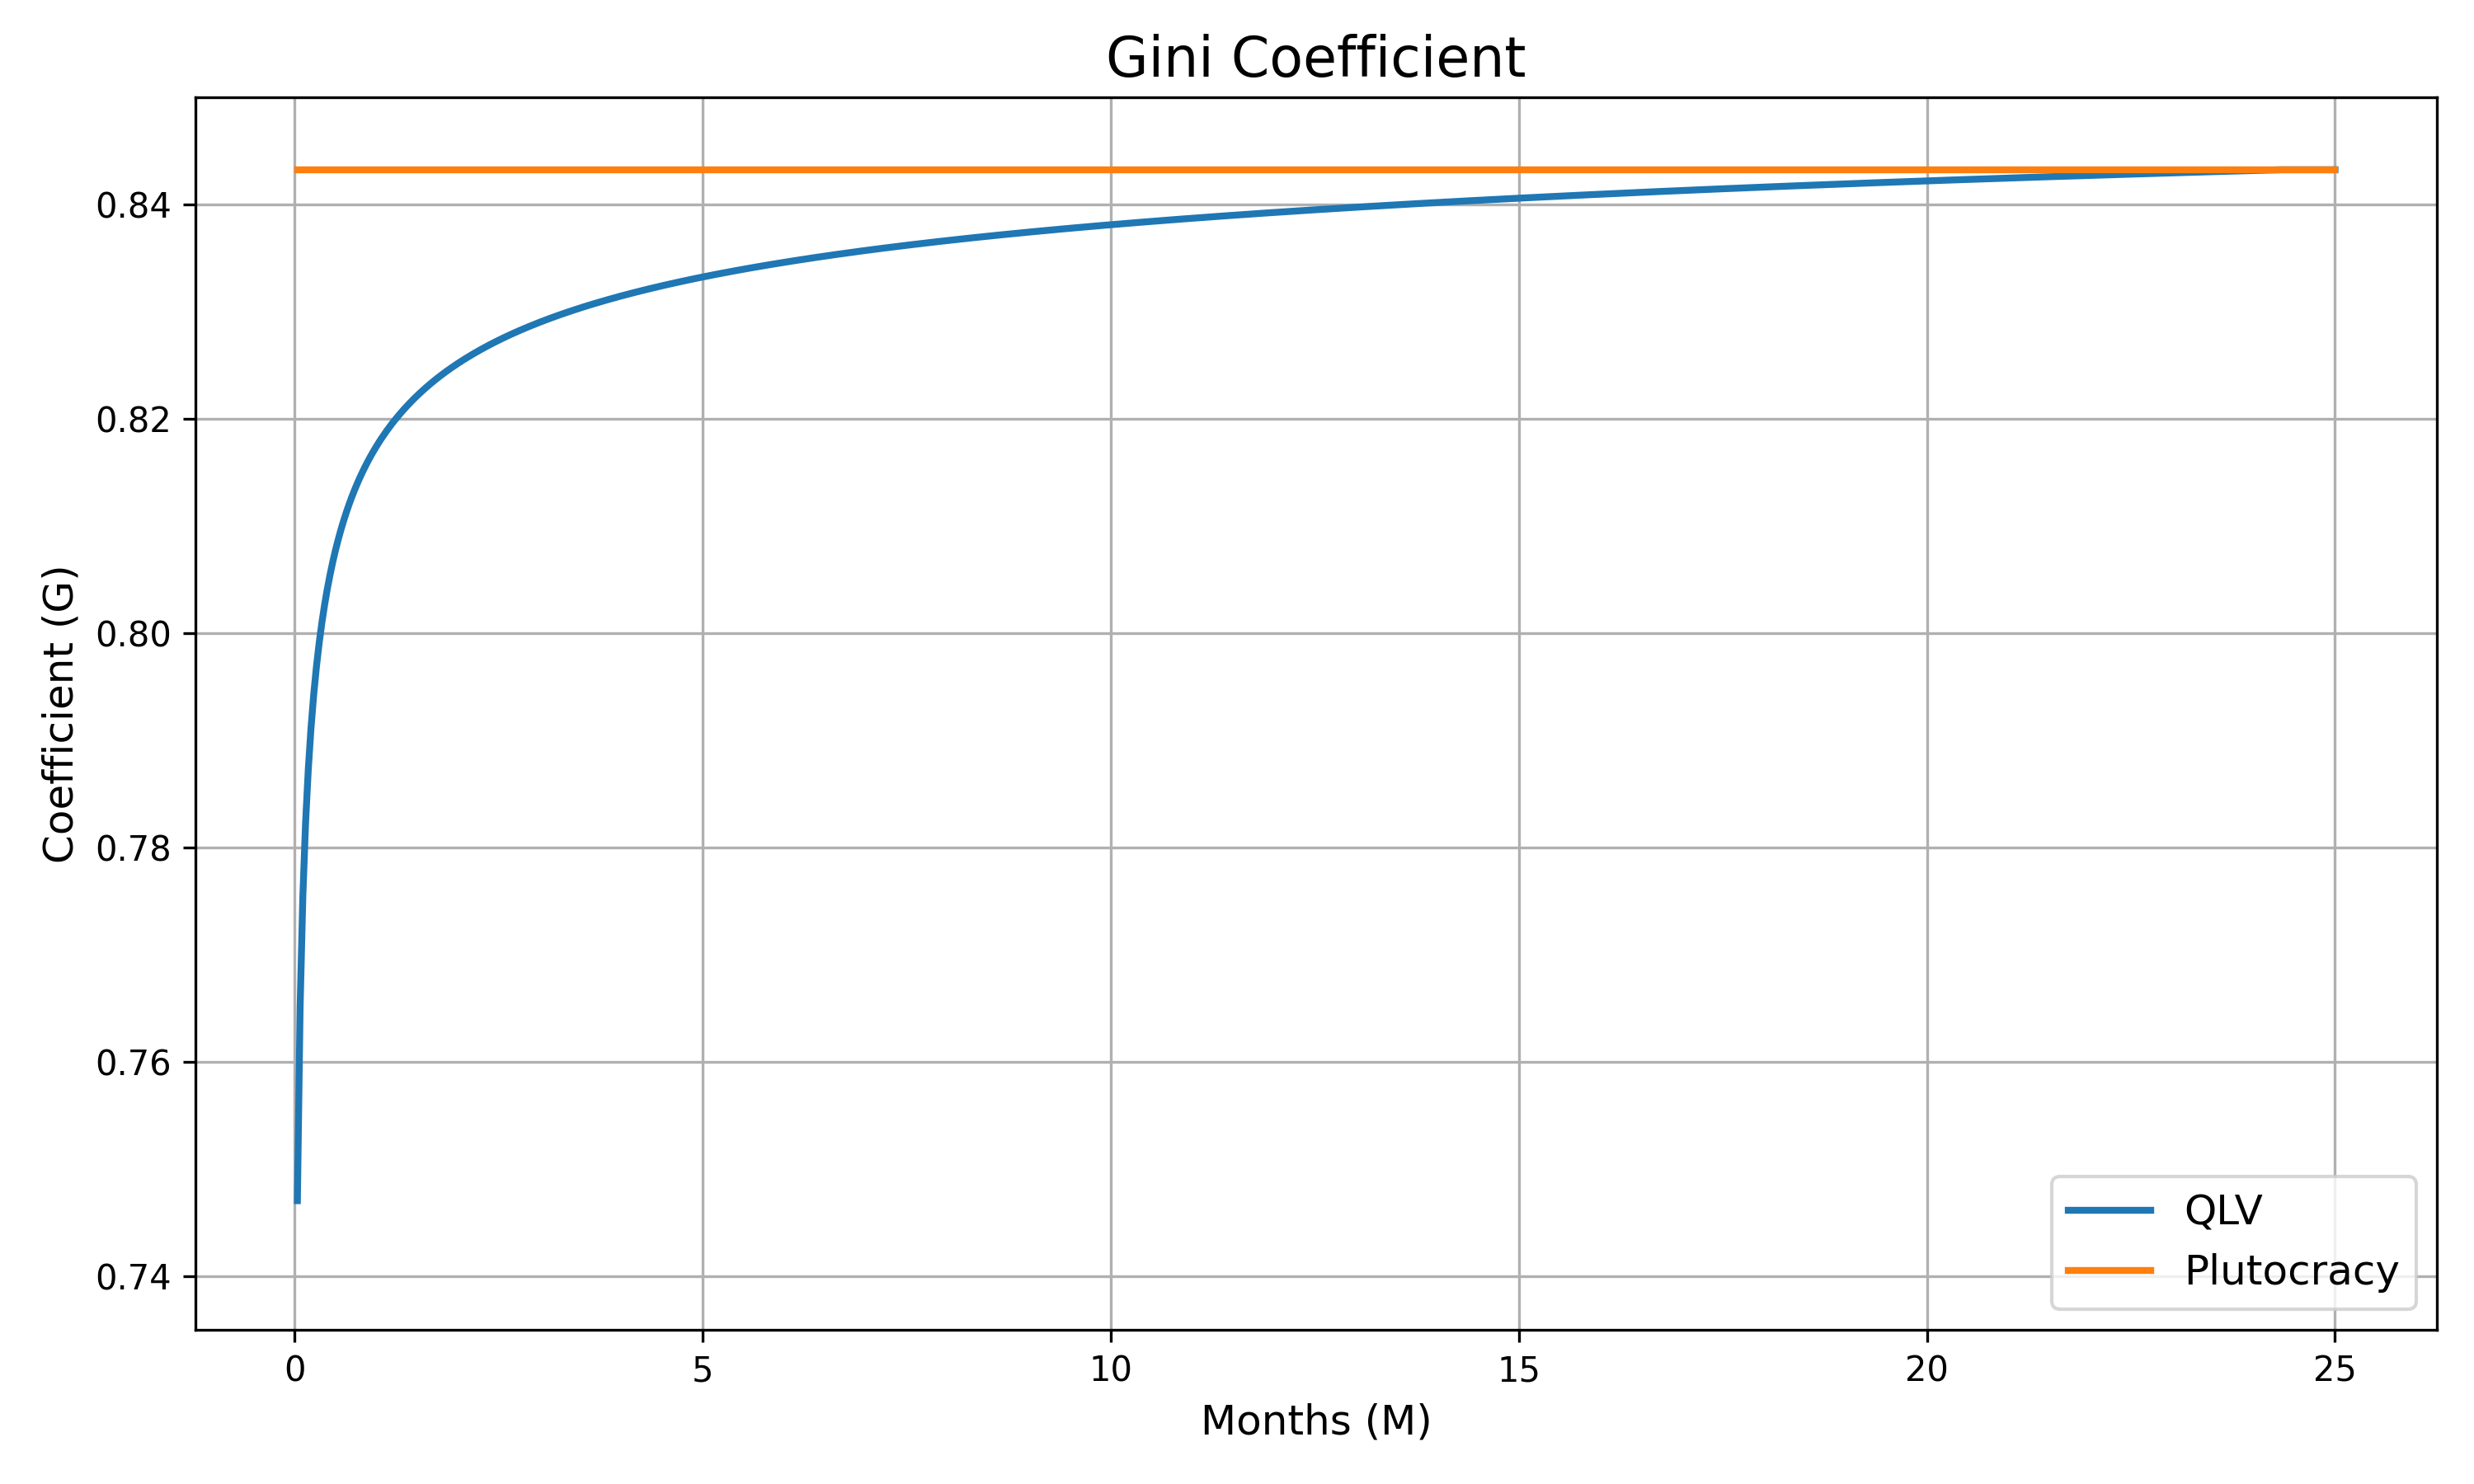
\includegraphics[width=0.8\textwidth]{assets/gini_benchmark.png}
    \caption{Gini analysis of PV vs Plutocracy}
    \label{fig:gini}
\end{figure}

\subsection{Wealth Dispersion}

PV significantly empowers smaller stakeholders through the quadratic dampening in the early phases of the governance cycle. By using the Gini coefficient, we can investigate how much of an impact this has.Assuming the previous distribution defined in the voting power plot, we can see that it effectively empowers minor demographics in the early and median phases of the voting power curve until converging towards purely linear weighting.

\subsection{Coalition building}
By introducing opacity in power progression, the model naturally incentivises cooperation, where participants within similar time-weighted tranches find strategic alignment. This creates an emergent governance landscape where shared experience and comparable power levels encourage collaborative strategies.  

\subsection{Graduated proposals}
Given the nature of the nuance of voting demographics in PV, the only logical decision to replicate that on the application layer is through tiered proposals by severity. Each with equivalent quorum and duration parameters to match, this mediates any short term advantages in voting power for any critical decisions through continuous voting periods plus caters to agile and effective decision making for lower severity ballots. 

\section{On Delegation}

 While vote buying in stakeholder governance has long been scrutinized, PV's time-stratified structure transforms these dynamics by creating significant friction for governance attacks. Unlike pure plutocracy where 51\% control requires acquiring tokens equivalent to that voting threshold, PV delegation attacks face compounding constraints: limited market depth as operational allocations are typically non-delegable, fragmented negotiations across stakeholders with heterogeneous time weights, and temporal requirements where high-influence votes must be developed over extended periods rather than purchased instantly. This creates indirect economic incentives for voter participation while substantially increasing coordination complexity and sustained costs for manipulation attempts, shifting governance attacks from capital allocation problems to multi-period coordination challenges with significantly higher execution risk.

\section{Conclusion}

Polycentric voting is a governance model to align the interests of an organisation with its participants and makes power dynamics explicit, rather than opaque, creating more strategic and nuanced governance. \\\\
It provides a more robust and efficient voting model for organisations versus pure plutocracy and is the closest mathematical representation of human decision-making, commitment, and loyalty within organisational systems.

\section{References}

[1] Lalley, Posner, E. Glen Weyl. "Democracy Squared” Journal of Political Economy 126 \\

[2] Ostrom, E. (1990). "Governing the Commons" The Evolution of Institutions for Collective Action. Cambridge University Press.

\end{document}